The upcoming LHC Run 3 will require more resources than the Worldwide LHC
Computing Grid (WLCG) can provide. Currently, PanDA WMS uses more than 300,000
cores at over 100 Grid sites, with a peak performance of 0.3 petaFLOPS. This
capacity will be sufficient for the planned analysis and data processing, but it
will be insufficient for the Monte Carlo production workflow and any extra
activity. To alleviate these challenges, ATLAS is expanding the current
computing model to include additional resources such as the opportunistic use of
supercomputers.

Generally, supercomputers are designed to support parallel computation that
requires runtime communication. Jobs are executed across multiple cores, each
core calculating a small part of the problem and communicating with other cores
via MPI. Accordingly, supercomputers have large number of worker nodes,
connected through a high-speed, low-latency dedicated network. Each worker node
has multicore CPUs, usually augmented with Graphics Processing Units (GPUs) or
other specialized coprocessors.

PanDA WMS has been designed to support distributed Grid computing. Executing
ATLAS workloads or workflows involves concurrent and/or sequential runs of
possibly large amount of jobs, each requiring no or minimal parallelization and
no runtime communication. Thus, computing infrastructure like WLCG have been
designed to aggregate large amount of computing resources across multiple sites.
While each site may deploy MPI capabilities, usually these are not used to
perform distributed computations.

We developed and deployed a single-point solution to better understand the
problem space of enabling a WMS designed for HTC to execute production workflows
on resources designed to support HPC. The PanDA team developed a job broker to
support the execution of part of the ATLAS production Monte Carlo workflow on
Titan, a leadership-class supercomputer managed by the Oak Ridge Leadership
Computing Facility (OLCF) at the Oak Ridge National Laboratory (ORNL).


% -----------------------------------------------------------------------------
\subsection{Architectures and Interfaces}
\label{ssec:panda-titan}

The Titan supercomputer, current number three on the Top 500 list~\cite{top500},
is a Cray XK7 system with 18,688 worker nodes and a total of 299,008 CPU cores.
Each worker node has an AMD Opteron  6274 16-core CPU, a Nvidia Tesla K20X GPU,
32 GB of RAM and no local storage, though a 16 GB RAM disk can be set up. Work
nodes use Cray’s Gemini interconnect for inter-node MPI messaging. Titan is
served by the Spider II~\cite{oral2013olcf}, a Lustre filesystem with 32 PB of
disk storage, and by a 29 PB HPSS tape storage system. Titan’s worker nodes run
Compute Node Linux, a run time environment based on SUSE Linux Enterprise
Server.

Titan's users submit jobs to Titan's PBS scheduler by logging into login or data
transfer nodes (DTNs). Titan's authentication and authorization model is based
on two-factor authentication with a RSA SecurID key. Login nodes and DTNs have
out/inbound wide area network connectivity while worker nodes have only local
network access. Fair-share and allocation policies are in place both for the PBS
batch system and shared file systems.

Titan's architecture, configuration and policies poses several challenges to the
integration with PanDA. The default deployment
model of PanDA Pilot is unfeasible on Titan: PanDA Pilot is required to contact
the Job Dispatcher of the PanDA Server to pull jobs to execute, but this is not
possible on Titan because worker nodes do not offer outbound network
connectivity. Further, Titan does not support PanDA's security model based on
certificates and virtual organizations, making PanDA's approach to identity
management also unfeasible. While DTNs offer wide area network data transfer, an
integration with ATLAS DDM is beyond the functional and administrative scope of
the current prototyping phase. Finally, the specific characteristics of the
execution environment, especially the absence of local storage on the worker
nodes and modules tailored to Compute Node Linux, require re-engineering of
ATLAS application frameworks.

Currently, very few HEP applications can benefit from Titan's GPUs but some
computationally-intensive and non memory-intensive tasks of ATLAS workflows can
be off-loaded from the Grid to Titan's. Further, when HEP tasks can be
partitioned into independent jobs, Titan worker nodes can be used to execute up
to 16 concurrent payloads, one per each available core. Given these constraints
and challenges, the type of task most suitable for execution at the moment on
Titan is Monte Carlo detector simulation. This type of task is mostly
computational-intensive, requiring less than 2GB of RAM at runtime and with
small input data requirements. Detector simulation tasks in ATLAS are performed
via AthenaMP~\cite{aad2010atlas}, the ATLAS software framework integrating the
GEANT4 simulation toolkit~\cite{agostinelli2003geant4}. These tasks account for
$\approx$ 60\% of all the jobs on WLCG, making them a primary candidate for
offloading.

Detector simulation is part of the ATLAS production Monte Carlo (MC)
workflow~\cite{rimoldi2006atlas,de2013delphes,ritsch2014atlas}. The MC workflow
consists of four main stages: event generation, detector simulation,
digitization, and reconstruction. Event generation creates sets of particle
four-momenta via different generators, e.g., PYTHIA~\cite{sjostrand2006pythia},
HERWIG~\cite{corcella2001herwig} and many others. The detector simulator is
called Geant4~\cite{agostinelli2003geant4} and simulates the ATLAS detector and
the interaction between that detector and particles. Each interaction creates a
so-called hit and all hits are collected and passed on for digitalization, where
hits are further processed to mimic the readout of the detector. Finally,
reconstruction operates local pattern recognition, creating high-level objects
like particles and jets.

% -----------------------------------------------------------------------------
\subsection{PanDA Broker}
\label{ssec:panda_titan}

The lack of wide area network connectivity on Titan's worker nodes is the most
relevant challenge for integrating PanDA WMS and Titan. Without connectivity,
Panda Pilots cannot be scheduled on worker nodes because they would not be able
to communicate with PanDA Server and therefore pull and execute jobs. This makes
impossible to port PanDA Pilot to Titan while maintaining the defining feature
of the pilot abstraction: decoupling resource acquisition from workload
execution via multi-stage scheduling.

The unavailability of pilots is a potential drawback when executing distributed
workloads like MC detector simulation. Pilots are used to increase the
throughput of distributed workloads: while pilots have to wait in the
supercomputer's queue, once scheduled, they can pull and execute jobs
independent from the system's queue. Jobs can be concurrently executed on
every core available to the pilot, and multiple generations of concurrent
executions can be performed until the pilot's walltime is exhausted. This is
particularly relevant for machines like Titan where queue policies privilege
parallel jobs on the base of the number of worker nodes they request: the higher
the number of nodes, the shorter the amount of queue time (modulo fair-share and
allocation policies).

The backfill optimization of Titan's Moab scheduler allows to avoid the overhead
of queue wait times without using pilot abstraction~\cite{maui_backfill_url}.
With this optimization, Moab starts low-priority jobs when they do not delay
higher priority jobs, independent of whether the low-priority jobs were queued
after the high-priority jobs.

When the backfill optimization is enabled, users can interrogate Moab about the
number of worker nodes and walltime that would be available to a low-priority
job at that moment in time. If a job is immediately submitted to Titan with that
number of worker nodes and walltime, chances are that Moab will immediately
schedule it, reducing its queue time to a minimum. In this paper, we call this
number of worker nodes and walltime an available `backfill slot'.

Compared to pilots, backfill has the disadvantage of limiting the amount of
worker nodes that can be requested. Pilots are normal jobs: they can request as
many worker nodes and walltime as a queue can offer. On the contrary, jobs sized
according to an available backfill slot depend on the number of worker nodes and
walltime that cannot be given to any other job at that moment in time.

At any point in time, the size of an available backfill slot is typically a
small fraction of the total capacity of a resource. Notwithstanding, given the
size of Titan this translates into a substantial capacity. Every year, about
10\% of Titan's capacity remains unused~\cite{barker2016us}, corresponding to an
average of 30,000 unused cores (excluding GPU cores). This equals to roughly
10\% of the overall capacity of WLCG.

Given the communication requirements of PanDA Pilots and the unused capacity of
Titan, PanDA pilot was repurposed to serve as a job broker on the DTN nodes of
Titan (Fig.~\ref{fig:panda_broker}). Maintaining the core modules of PanDA Pilot
and its stand-alone architecture, this prototype called `PanDA Broker'
implements functionalities to: (i) interrogate Titan about backfill
availability; (ii) pull ATLAS jobs and events from PanDA Server; (iii) wrap the
payload of ATLAS jobs into MPI scripts; (iv) submitting MPI scripts to Titan's
PBS batch system and monitor their execution; and (v) staging and preparing
input/output files. Backfill querying, payload wrapping, and scripts submission
required a new implementation while pulling ATLAS job and events, and file
staging were inherited from PanDA Pilot.

Backfill querying is performed via a dedicated Moab scheduler command while a
tailored Python MPI script is used to execute the payload of ATLAS jobs. This
MPI script enables the execution of unmodified Grid-centric, ATLAS jobs on
Titan. Typically, a MPI script is workload-specific as it sets up the execution
environment for a specific payload. This involves organization of worker
directories, data management, optional input parameters modification, and
cleanup on exit. Upon submission, a copy of the MPI script runs on every
available worker node, starting the execution of the ATLAS job's payload in a
subprocess and waits until its completion.

MPI scripts are submitted to Titan's PBS batch system via
RADICAL-SAGA~\cite{radical-saga_url}, a Python module, compliant with the OGF
GFD.90 SAGA specification~\cite{goodale2008simple}. The Simple API for Grid
Applications (SAGA) offers a unified interface to diverse job schedulers and
file transferring services. In this way, SAGA provides an interoperability layer
that lowers the complexity of using distributed infrastructures. Behind the API
façade, RADICAL-SAGA implements a adaptor architecture: each adaptor interface
the SAGA API with different middleware systems and services, including the PBS
batch scheduler of Titan.

The data staging capabilities of the PanDA Broker are implemented via a file
system that is shared among DTNs and worker nodes. The input files with the
events of the ATLAS jobs are downloaded on the shared filesystem from the data
center of Brookhaven National Laboratory (BNL). The MPI script setup process
includes making the location of these files available to the payload of the
ATLAS's jobs. The PanDA Broker can locate the payload's output files on the
shared filesystem and transfer them from Titan BNL.

Once deployed on Titan, every PanDA Broker supports the execution of MC detector
simulations in 9 steps. PanDA Broker queries the Job Dispatcher module of the
PanDA server for ATLAS jobs that have been bound to Titan by JEDI
(Fig.~\ref{fig:panda_broker}:1). Upon receiving jobs descriptions, PanDA Broker
pulls jobs' input files from BNL to the OLCF Lustre file system
(Fig.~\ref{fig:panda_broker}:2). PanDA Broker queries Titan's Moab scheduler
about the current available backfill slot (Fig.~\ref{fig:panda_broker}:3) and
creates an MPI script, wrapping enough ATLAS jobs' payload to fit the backfill
slot. PanDA Broker submits the MPI script to the Titan's Torque batch system via
RADICAL-SAGA (Fig.~\ref{fig:panda_broker}:4).

Upon execution on the worker node(s) (Fig.~\ref{fig:panda_broker}:5), the MPI
script initializes and configures the execution environment
(Fig.~\ref{fig:panda_broker}:6), and executes one AthenaMP for each available
work node (Fig.~\ref{fig:panda_broker}:7). AthenaMP retrieves events from Lustre
(Fig.~\ref{fig:panda_broker}:8) and spawns 1 Geant4 event simulation process on
each of the 16 available cores (Fig.~\ref{fig:panda_broker}:9). Upon completion
of each MPI script, PanDA Broker transfer the jobs' output to BNL
(Fig.~\ref{fig:panda_broker}:10), and performs cleanup.

While PanDA Broker implementation is resource specific, it was successfully
ported to other supercomputers, including the HPC2 at the National Research
Center ``Kurchatov Institute'' (NRC-KI)~\cite{belyaev2015integration},
Edison/Cori at the National Energy Research Scientific Computing Center
(NERSC)~\cite{barreiro2016panda}, and SuperMUC at the Leibniz Supercomputing
Centre (LRZ)~\cite{barreiro2016panda}.

\begin{figure}
    \centering
    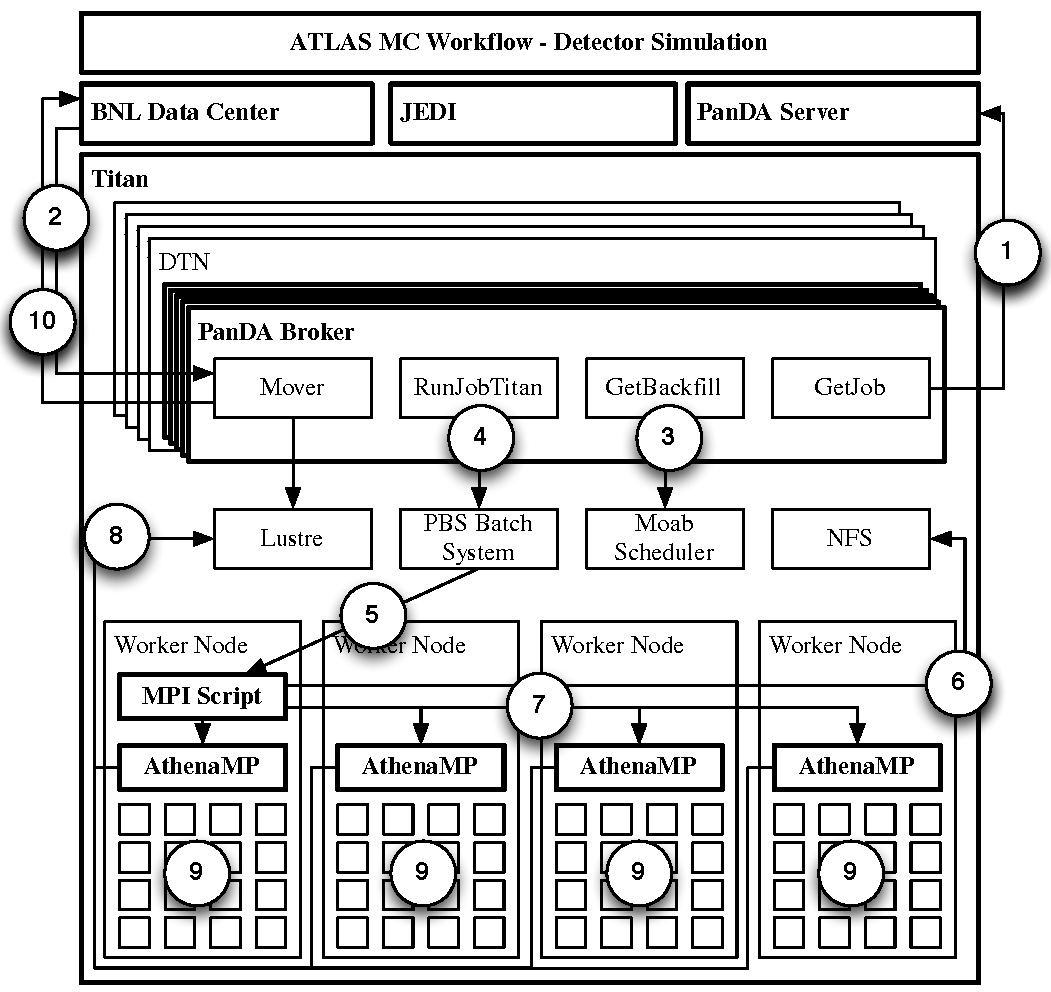
\includegraphics[width=\columnwidth]{figures/panda_broker_architecture.pdf}
    \vspace{-0.3in}
    \caption{PanDA Broker architecture as deployed on Titan. Numbers indicates
    the execution process of a detector simulation job, part of the production
    ATLAS MC workflow.}
\label{fig:panda_broker}
\end{figure}
\vspace{-0.04in}
